\section{Experimental Evaluation}

This section evaluates the scale and performance of our prototype using a mix of
metadata-intensive and data-intensive benchmarks. Our evaluation layers \sys on
the Panasas PanFS file system, and focuses on three questions:
\begin{itemize}
\item How does \sys enhance metadata throughput, particularly
number of file creates per second for concurrent file creation workloads, on
the PanFS storage system?
\item What is the data throughput of \sys layered on PanFS for N-N checkpointing 
workload found in HPC systems?
\item How portable is \sys to be used on other cluster storage systems and
configurations?
\end{itemize}

\subsection{Setup and Methodology}

Our prototype is implemented in about 10,000 lines of C code using
a modular design comprising of \tfs, \ldb and PanFS layers. In particular, the
PanFS layer is unmodified and can be replaced with any other cluster file
system. The current version implements most common POSIX file system operations 
except \texttt{hardlink}, \texttt{rename}, and \texttt{xattr} related operations.
The first two operations, \texttt{hardlink} and \texttt{rename}, are
particularly complicated because they need distributed transaction support for
correct and fault tolerant cross-server operations; this problem is beyond the
scope of this paper.

All experiments were performed on two clusters described in Table
\ref{tab:setting}. The first cluster is a 5-shelf PanFS storage cluster, and the 
second cluster is a 64-node setup to run \sys code and applications.
Table \ref{tab:setting} describes the hardware and software configuration of
these clusters.
The first cluster is used to evaluate the scale and performance of the
underlying cluster file system that uses our middleware.
The second cluster is used to demonstrate that our middleware 
solution can be layered on other file system deployments without any
configuration changes; this setup
emulates a case that each GIGA+ server runs in a different NFS node and manages 
its own \tfs instance locally to scale the metadata performance of NFS.
In all tests, the client uses library version code;
the threshold for splitting a partition is always 8,000 entries;
and \tfs managed by GIGA+ server syncs its data every 5 seconds.

\begin{footnotesize}
\begin{table}
\begin{tabular}{lcc}
\toprule
      & Cluster 1 & Cluster 2 \\
      & (Storage cluster) & (Test applications)\\
\midrule
\#Nodes & 5 & 64 \\
\hline
OS &   CentOS 6.3 &  Ubuntu 12.10 \\
Kernel & 2.6.32 x86\_64 & 3.6.6 x86\_64 \\
\hline
CPU & AMD Opteron 6272 &  AMD Opteron 242 \\
    & 64 Cores & Dual Core\\
\hline
Memory & 128GB DDR &  16GB DDR \\
\hline
Network & 40GE NIC &  1GE NIC  \\
\hline
Storage & PanFS & Western Digital \\
System &      5 Shelves & Local hard disk  \\
       &   (5 MDS + 50 ODS) &  2TB per node  \\
\hline
& & 100 seeks/sec \\
& & random seeks   \\
& & 137.6 MB/sec  \\
& & seq. reads    \\
& & 135.4 MB/sec  \\
& & seq. writes   \\
\bottomrule \\
\end{tabular}
\caption{
\textit{\footnotesize Settings of two clusters used for evaluation.}
}
\label{tab:setting}
\end{table}
\end{footnotesize}

In the following sections, we will first show the evaluation
on the end-to-end performance of the integrated system on top of PanFS,
and then present the results of a scaling experiment on another platform.

\subsection{End-to-end System Evaluation}
\label{sec:fullsystem}
We performed an end-to-end evaluation of our prototype in a cluster with 5 test nodes.
The cluster is connected to a 5-shelves PanFS storage system
with 5 metadata nodes and 50 storage nodes.
Since each test node has 64 cores and a 40GE NIC, they are able to
to saturate the data bandwidth of our PanFS storage cluster.
Because of some technique difficulties,
we did not run our GIGA+ server processes inside the metadata node.
Instead, we co-locate our GIGA+ server processes
with client processes in the test nodes.
Each test node runs a GIGA+ server that is assigned to a metadata node
as explained in Section \ref{design.integration}.
We ran a series of HPC benchmarks (used by parallel file system vendors and users)
to test metadata path and data path separately,
including the open source \textit{mdtest} synthetic benchmark \cite{mdtest}
and File System Test Suite checkpoint benchmark from LANL \cite{mpiio}

\textbf{Metadata Intensive Workloads -- }
We used the synthetic mdtest benchmark \cite{mdtest}
to generate a three-phase workload:
The first phase is to create 5 million
zero-files in a single shared directory \cite{ceph:weil06, GIGA11};
the second phase is to perform $stat()$ on random files in the directory;
the third phase is to delete all the files in the directory in a random order.
Each phase involves multiple clients to issue the operations concurrently.

If we directly use the above workload to directly compare our layered system
against the original PanFS, it would not be fair enough.
This is because a single directory can only use the hardware resource
of one metadata manager in PanFS,
and PanFS also limits a single directory to 1 million files.
Therefore we chose to compare native PanFS creating 1 million files
in 5 different directories owned by 5 different metadata managers.
The total number of clients used for testing the two systems
are kept the same.

\begin{figure}[t]  %%%%%%%%%%%%%%%%%%%%%%%
\centerline{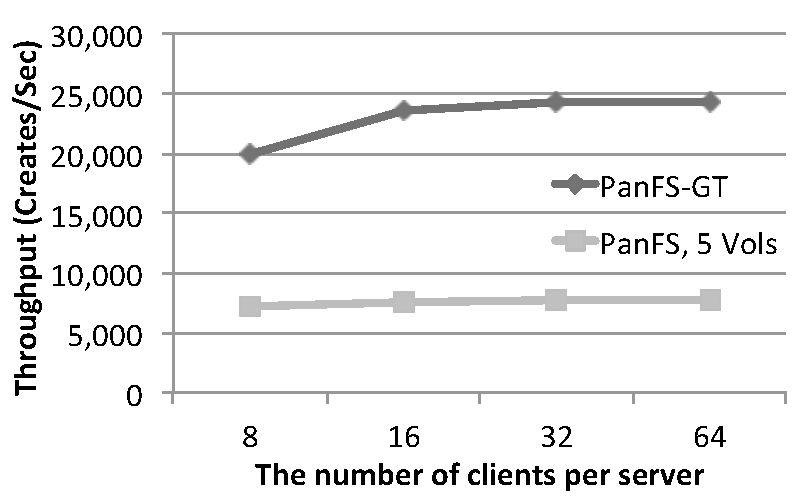
\includegraphics[scale=0.7]{./figs/zero_file_creation_on_panfs}}
\vspace{10pt}
\caption{\normalsize
\textit{Average throughput during creating five million zero-length files
in one empty directory with different number of clients per test node.
Running 32 and more clients per test node is able to saturate \sys
and original PanFS}
}
\vspace{10pt}
\hrule
\label{graph:creation_clients}
\end{figure}       %%%%%%%%%%%%%%%%%%%%%%%

\begin{figure}[t]  %%%%%%%%%%%%%%%%%%%%%%%
\centerline{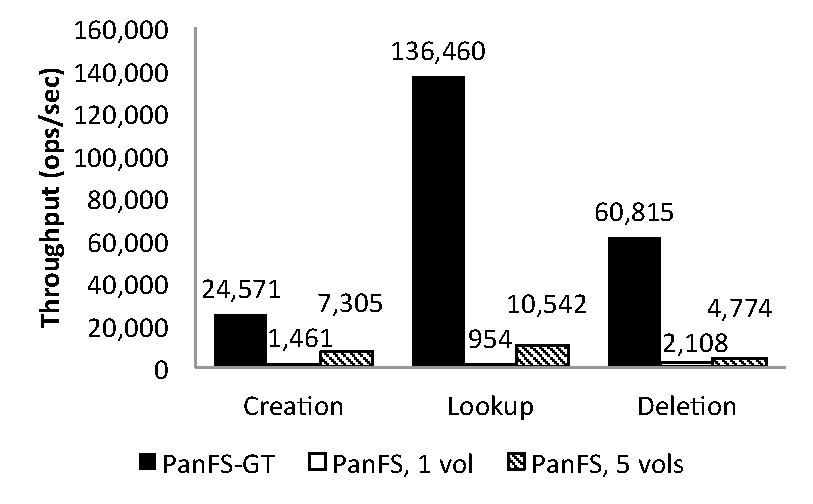
\includegraphics[scale=0.7]{./figs/mdtest}}
\vspace{10pt}
\caption{\normalsize
\textit{mdtest:
The average aggregated throughput of different operations in mdtest
when generating 5 million zero-length files in a single shared directory.
Since PanFS has a hard limit to allow only create 1 million entries
in one directory, the bar showing PanFS with 1 volume only gives
the average throughput for the case of creating 1 million entries.
}
}
\vspace{10pt}
\hrule
\label{graph:mdtest_ops}
\end{figure}       %%%%%%%%%%%%%%%%%%%%%%%


Figure \ref{graph:creation_clients} shows the aggregated througphut during
the first phase. We varies the nubmer of clients running in each test node
to find the right number that can saturate both systems.
Both systems achieve the highest aggregated throughput when the number
of clients per node is 32 or more. In all the experiments shown later,
we present the results with 32 clients per test node if without explanation.
For all cases, \sys  is approximately 3.5 times faster than the native PanFS
using 5 volumes. The aggregated throughput with 32 clients per server
achieves about 24,571 creation per second.

Figure \ref{graph:mdtest_ops} shows the aggregated througphut of
different operations during three phases in mdtest.
Besides \sys and PanFS using 5 volumes, it also shows
the aggregated throughput of creating 1 million files in one volume of PanFS.
For $lookup$ and $deletion$ workloads,
\sys gains more advantages over original PanFS,
and achieves about 10 to 15 times speed up.
Fast lookup is due to the memory indexing and Bloom filters in \ldb.
For deletion of a key, \ldb essentially just inserts the key and a deletion mark
into its memtable, and delays the actual deletion in later compaction processes.


\textbf{Small File Workloads -- }
We also use mdtest benchmark to generate files with small size data to evaluate
the effectiveness of embedding file content with the metadata inside \tfs.
Similar to the previous test,
mdtest benchmark creates 5 million files in a single directory
but with file data of two different sizes: 4KB and 16 KB.
4KB is the median file size for many desktop workloads \cite{Bill11},
and 16KB is the median file size for some large storage clusters using PanFS \cite{brent13}.
The threshold $T$ for our prototype is set to 64KB, so all these files
are stored in \tfs instance.

%compaction and CPU usage
Figure \ref{graph:smallfiles} shows the aggregated throughput during the test,
which is aggregated from all clients. For 4KB file size,
\sys is about $2.5\times$ faster than original PanFS.
However, \sys is about $35\%$ slower than PanFS for 16KB file size.
We found that embedding 16KB file makes the key-value pair significanly larger,
and causes higher write amplification during compaction process in \ldb,
since \ldb tries to merge sort both file data and metadata.
Additionally, \ldb will firstly write the inserted key-value pairs
to the transaction log, and then (during a compaction) to the SSTable.
With larger key-value pairs, LevelDB's per-operation efficiency is
slowed down by the cost of extra copies of large values.
This suggests that the threshold $T$ for embedding file size should not be
greater than 16 KB. For larger embedding file size,
we might sacrafice the read performance to maitain its fast insertion rate
by using column-based approach which stores metadata and small file separately.
Such investigation is left for future works.

\begin{figure}[t]  %%%%%%%%%%%%%%%%%%%%%%%
\centerline{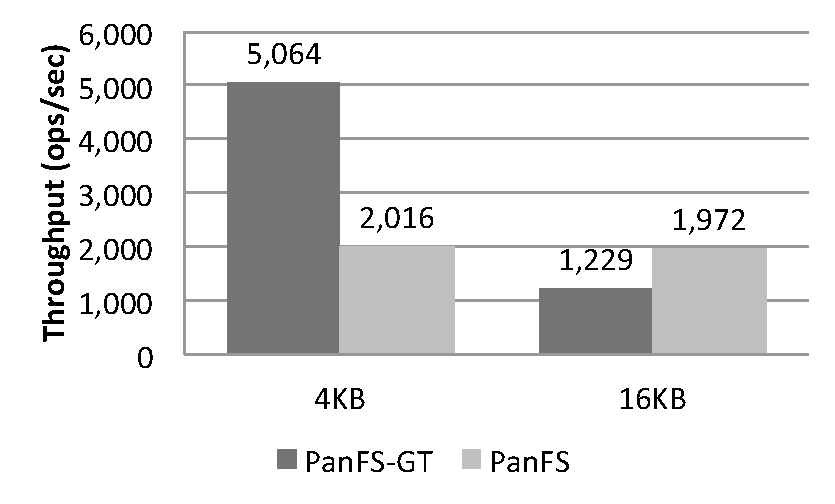
\includegraphics[scale=0.7]{./figs/small_file_creates}}
\vspace{10pt}
\caption{\normalsize
\textit{Average aggregated throughput during creating 5 million small files
with different size in one shared directory}
}
\vspace{10pt}
\hrule
\label{graph:smallfiles}
\end{figure}       %%%%%%%%%%%%%%%%%%%%%%%


%Library version not FUSE
%Clean cache

\textbf{Data Intensive Workloads -- }
The LANL filesystem checkpoint benchmark can
generate many types for HPC checkpoint I/O patterns.
For our test purposes, we configured the benchmark to generate
a concurrent N-N checkpoint write and read workload.

All checkpoint file I/O is performed by a set of processes
that synchronize with each other using MPI barriers.
At the begining, each process opens a freshly created checkpoint file
for writing and then waits at a barrier until all processes are ready to write.
Once all processes are ready, each processes starts
concurrently writing the checkpoint data to its own file,
until it has written the specified number of bytes.
It then waits barrier for all the other processes to finish writing,
and finally syncs its data to the file system and closes the file.
Before starting the read phase we terminate all processes
accessing these checkpoint files so that
we can unmount the filesystem in order to ensure that
all freshly written data has been flushed out from all the nodes' memory
to prevent caching from unfairly biasing our read performance.
After the filesystem has been mounted and restarted,
the benchmark reads the checkpoint in the same way it was written,
however we shift, so each process will read
the file generated by another process.

In this test, we also vary the number of clients per test node
from 8 to 64 clients. The clients in each node will generate
640GB checkpoint data in total to the underlying file system,
no mater what number of clients each node has.
The size of data buffer for each file system call is set to be 16KB.
For \sys, the checkpoint files generated in the test will be
first stored in \tfs, and the migrated to the underlying PanFS.

Figure \ref{graph:checkpoint_write} and \ref{graph:checkpoint_read}
show the average throughput during the write phase and read phase
in the N-N checkpoint workload respectively. We can see \sys
performs comparably with the native PanFS.
For read checkpoint worload, the largest performance loss is less than $10\%$.
And \sys is even faster in write checkpoint phase.
The embedding of small files do not affect the data transferring
of large files.

\begin{figure}[t]  %%%%%%%%%%%%%%%%%%%%%%%
\centerline{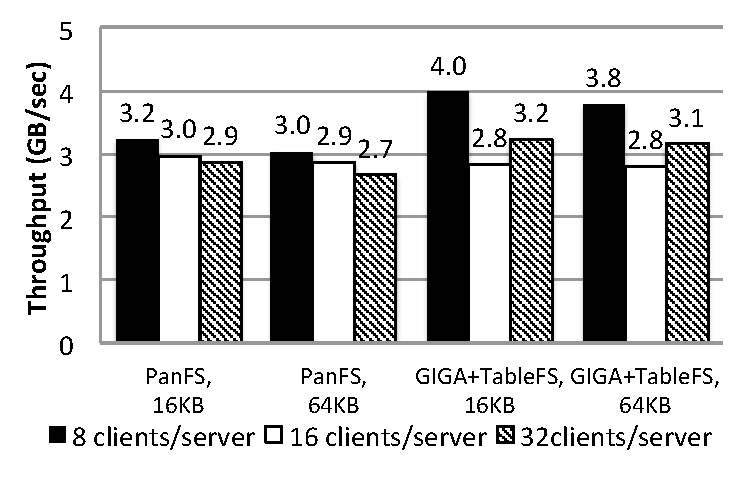
\includegraphics[scale=0.7]{./figs/checkpointing_write}}
\vspace{10pt}
\caption{\normalsize
\textit{
The aggregated write throughput in N-N check-pointing workload.
Each volume receives 640 GB data.
}
}
\vspace{10pt}
\hrule
\label{graph:checkpoint_write}
\end{figure}       %%%%%%%%%%%%%%%%%%%%%%%

\begin{figure}[t]  %%%%%%%%%%%%%%%%%%%%%%%
\centerline{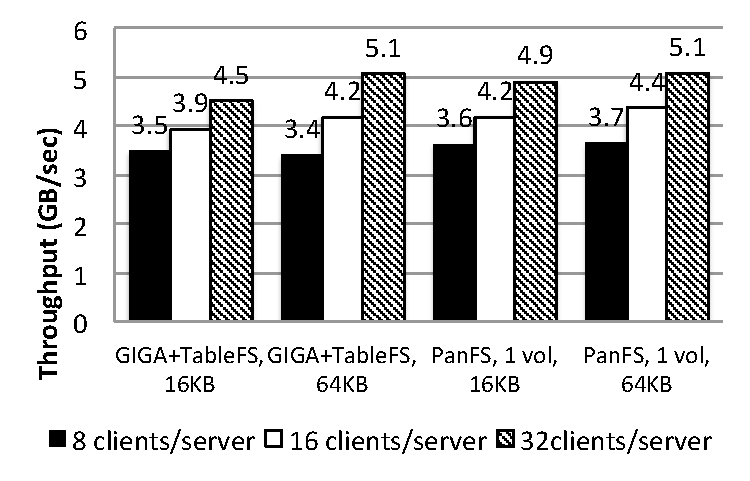
\includegraphics[scale=0.7]{./figs/checkpointing_read}}
\vspace{10pt}
\caption{\normalsize
\textit{
The aggregated read throughput in N-N check-pointing workload.
}
}
\vspace{10pt}
\hrule
\label{graph:checkpoint_read}
\end{figure}       %%%%%%%%%%%%%%%%%%%%%%%



\subsection{Understanding Scaling Behavior}

\begin{figure*}[t]
\centerline{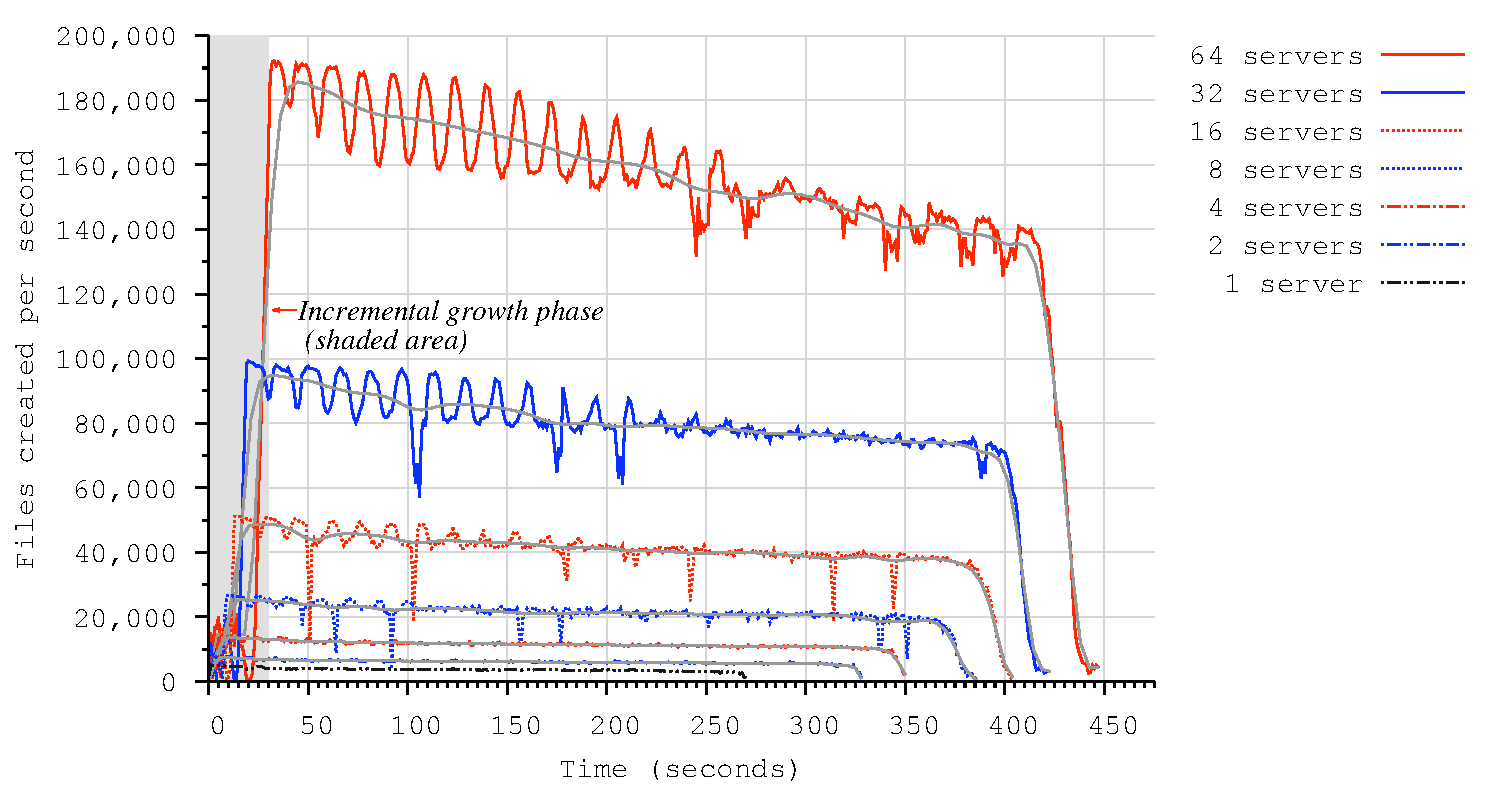
\includegraphics[scale=0.55]{./figs/ldb_insertrate}}
\vspace{10pt}
\caption{\textit{\footnotesize 
Our middleware metadata service prototype shows promising scalability
up to 64 servers.
Note that at the end of the experiment,
the throughput drops to zero
because clients stop creating files as they finish 1 million files per client.
(Solid lines are Bezier curves to smooth the variability.)
}
}
%\vspace{10pt}
\hrule
\label{graph:ldb-scaling}
\end{figure*}

This section shows how \sys scales over time in large multi-server setup. To
understand this behavior we layered \sys on a different cluster (cluster \#2
from Table \ref{tab:setting}) comprising of 64-nodes running \sys clients and
servers. The main difference is the backend storage: this analysis emulates a
federated NFS setup where each \psys server process in node manages its own \tfs 
instance and store SSTables into a local disk.
To emulate shared storage for split operations, we used a NFS-mounted shared 
directory accessible from all machines; this shared directory was only used for 
moving SSTables of splitting directory partitions across servers.
%The distributed logging is not available in this experiment setting,
%but which does not limit testing the scalability of our system.

This analysis uses a \textit{weak scaling} experiment that creates
1 million files per server, for a total of 64 million files in the
64-server configuration. We vary the number of servers from 1 to 64
to understand how performance scales with more servers.

Figure \ref{graph:ldb-scaling} shows the instantaneous throughput
during the concurrent create workload.
The main result in this figure is that as the number of servers doubles the
throughput of the system also scales up. With 64 servers, \giga can achieve a
peak throughput of about 190,000 file creates per second.
The prototype delivers peak performance after the directory workload
has been spread among all servers.
Reaching steady-state, the throughput quickly grows
due to the splitting policies adopted by \giga.


After reaching the steady state, throughput slowly drops
as \tfs builds a larger metadata store.
In fact, in large setups with 8 or more servers,
the peak throughput drops by as much as 25\% (in case of the 64-server setup).
This is because when there are more entries already existing in \tfs,
it requires more compaction work to maintain invariants inside \ldb
and to perform a negative lookup before each create
has to search more SSTables on disk.
In theory, the work of inserting a new entry to a LSM-tree is $O(\log_{B}(n))$
where $n$ is the total number of inserted entries, and $B$ is a constant factor
proportional to the average number of entries transferred in each disk request
\cite{Bender2007}.
Thus we can use the formula $\frac{a\cdot S+b}{\log{T}}$ to
approximate the throughput timeline in Figure \ref{graph:ldb-scaling},
where $S$ is the number of servers, $T$ is the running time,
and $a$ as well as $b$ are constant factors
relative to the disk speed and splitting overhead.
This estimation projects that when inserting 64 billion files with 64 servers,
the system may deliver an average of 1,000 operations per second per server,
i.e. 64,000 operations per second in aggregate.
This still exceeds today supercomputer's most rigorous scalability demands for
40,000 file creates per second in a single directory \cite{hpcs-io:2008}.

